%% tese_lncc.tex
%%
%% A última versão deste modelo está em
%%   https://github.com/equipe-customizacao-tese-lncc/tese_lncc
%%
%% Criado por:
%% Weslley da Silva Pereira
%% Lucas dos Santos Fernandez
%% Fortià Vila Verges
%%
%% Modificado por:
%% Equipe de customização - Fortià Vila Verges,
%%   Lucas dos Santos Fernandez, Weslley da Silva Pereira
%%
%% Este trabalho consiste de tese_lncc.tex,
%% abntex2lncc.sty e bibliografia.bib
%%

% ------------------------------------------------------------------------
% ------------------------------------------------------------------------
% Modelo de Trabalho Academico (tese de doutorado, dissertacao de
% mestrado e trabalhos monograficos em geral) em conformidade com
% ABNT NBR 14724:2011: Informacao e documentacao - Trabalhos academicos -
% Apresentacao
% ------------------------------------------------------------------------
% ------------------------------------------------------------------------

\documentclass[
	% -- opções da classe memoir --
	12pt,				% tamanho da fonte
	openright,			% capítulos começam em pág ímpar (insere página vazia caso preciso)
	oneside,			% para impressão em frente e verso use twoside
	a4paper,			% tamanho do papel.
	% -- opções da classe abntex2 --
	%chapter=TITLE,		% títulos de capítulos convertidos em letras maiúsculas
	%section=TITLE,		% títulos de seções convertidos em letras maiúsculas
	%subsection=TITLE,	% títulos de subseções convertidos em letras maiúsculas
	%subsubsection=TITLE,% títulos de subsubseções convertidos em letras maiúsculas
	sumario=tradicional,% sumário tradicional, com tabulação
	% -- opções do pacote babel --
	english,			% idioma adicional para hifenização
	french,				% idioma adicional para hifenização
	spanish,			% idioma adicional para hifenização
	brazil				% o último idioma é o principal do documento (mude se precisar)
	]{abntex2}

% ---
% Pacotes básicos
% ---
\usepackage{lmodern}			% Usa a fonte Latin Modern			
\usepackage[T1]{fontenc}		% Selecao de codigos de fonte.
\usepackage[utf8]{inputenc}		% Codificacao do documento (conversão automática dos acentos)
\usepackage{lastpage}			% Usado pela Ficha catalográfica
\usepackage{indentfirst}		% Indenta o primeiro parágrafo de cada seção.
\usepackage{color}			% Controle das cores
\usepackage{graphicx}			% Inclusão de gráficos
\usepackage{microtype} 			% para melhorias de justificação
\usepackage{abntex2lncc}		% Formatacao especifica do modelo do LNCC
% ---
		
% ---
% Pacotes adicionais, usados apenas no âmbito do Modelo Canônico do abnteX2
% ---
\usepackage{lipsum}				% para geração de dummy text
% ---

% ---
% Pacotes de citações
% ---
\usepackage[brazilian,hyperpageref]{backref}	 % Paginas com as citações na bibl
\usepackage[alf]{abntex2cite}	% Citações padrão ABNT
\usepackage{multirow}           % permite mesclar linhas e colunas em tabelas
\usepackage{pdfpages}		% Inclui p\'aginas PDF de documentos externos
\usepackage{amsmath,amssymb}	% Permite ambientes matem\'aticos e o uso do \eqref

% ---
% CONFIGURAÇÕES DE PACOTES
% ---

% ---
% Configurações do pacote backref
% Usado sem a opção hyperpageref de backref
\renewcommand{\backrefpagesname}{Citado na(s) página(s):~}
% Texto padrão antes do número das páginas
\renewcommand{\backref}{}
% Define os textos da citação
\renewcommand*{\backrefalt}[4]{
	\ifcase #1 %
		Nenhuma citação no texto.%
	\or
		Citado na página #2.%
	\else
		Citado #1 vezes nas páginas #2.%
	\fi}%
% ---

% ---
% CONFIGURAÇÕES DE USUÁRIO
% ---
	
% ---
% Pasta principal de imagens e logo do LNCC
\logoLNCC{lncc}
%{\centering 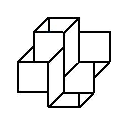
\includegraphics[scale=1.0]{lncc}}
% ---

% ---
% Tipo de trabalho (apenas uma das opções abaixo deve estar descomentada)
\dissertacaoMestrado
%\teseDoutorado
% ---

% ---
% Título
\titulo{Meu título}
% Nome do aluno
\nomeAutor{João da Silva}{Souza}
% Nome do orientador
\nomeOrientador{Pedro Costa}{dos Santos}
% Coorientador(es)
\coorientador{José Oliveira Pereira}
%\coorientador[Coorientadores:]{Coorientador 1 e Coorientador 2}
% ---

% ---
% Local
\local{Petrópolis, RJ - Brasil}
% Data
\data{Junho de 2016}
% Instituição
\instituicao{%
  Laboratório Nacional de Computação Científica
  \par
  Programa de Pós-Graduação em Modelagem Computacional}
% ---

% ---
% O preambulo deve conter o tipo do trabalho, o objetivo,
% o nome da instituição e a área de concentração
% portugues
\preambulo{\tipoTrabalho submetida ao corpo docente do Laboratório Nacional de Computação Científica como parte dos requisitos necessários para a obtenção do grau de \grau em Ciências em Modelagem Computacional.}
%ingles
%\preambulo{\tipoTrabalho submitted to the examining committee in partial fulfillment of the requirements for the degree of \grau of Sciences in Computational Modeling.}
% ---

% ---
% FICHA CATALOGRÁFICA
%
% Representa o código que sua tese/dissertação terá nos registros de  nossa biblioteca.
%
% Observação: Ao terminar de escrever sua tese/dissertação e a mesma for aprovada pela comissão de avaliação para a defesa, favor se dirigir a biblioteca.
% ---
\codebib{XXX.XXX}
\codetese{XXXX}
% ---

% ---
% Configurações de aparência do PDF final

\definecolor{blue}{RGB}{41,5,195}

% informações do PDF
\makeatletter
\hypersetup{
     	%pagebackref=true,
		pdftitle={\@title},
		pdfauthor={\@author},
    	pdfsubject={\imprimirpreambulo},
	    pdfcreator={LaTeX with abnTeX2},
		pdfkeywords={abnt}{latex}{abntex}{abntex2}{trabalho acadêmico},
		colorlinks=true,       		% false: boxed links; true: colored links
    	linkcolor=blue,          	% color of internal links
    	citecolor=blue,        		% color of links to bibliography
    	filecolor=magenta,      		% color of file links
		urlcolor=blue,
		bookmarksdepth=4
}
\makeatother
% ---

% ---
% Espaçamentos entre linhas e parágrafos
% ---

% O tamanho do parágrafo é dado por:
\setlength{\parindent}{1.3cm}

% Controle do espaçamento entre um parágrafo e outro:
\setlength{\parskip}{0.2cm}  % tente também \onelineskip

% ---
% compila o indice
% ---
\makeindex
% ---

% ----
% Início do documento
% ----

\begin{document}

% Seleciona o idioma do documento (conforme pacotes do babel)
%\selectlanguage{english}
\selectlanguage{brazil}

% Retira espaço extra obsoleto entre as frases.
\frenchspacing

% ----------------------------------------------------------
% ELEMENTOS PRÉ-TEXTUAIS
% ----------------------------------------------------------
% \pretextual

% ---
% Capa
% ---
\imprimircapa
% ---

% ---
% Folha de rosto
% (o * indica que haverá a ficha bibliográfica)
% ---
\imprimirfolhaderosto*
% ---

% ---
% Inserir a ficha bibliografica
% ---

% Isto é um exemplo de Ficha Catalográfica, ou ``Dados internacionais de
% catalogação-na-publicação''. Você pode utilizar este modelo como referência.
% Porém, provavelmente a biblioteca da sua universidade lhe fornecerá um PDF
% com a ficha catalográfica definitiva após a defesa do trabalho. Quando estiver
% com o documento, salve-o como PDF no diretório do seu projeto e substitua todo
% o conteúdo de implementação deste arquivo pelo comando abaixo:
%
% \begin{fichacatalografica}
%     \includepdf{fig_ficha_catalografica.pdf}
% \end{fichacatalografica}

\begin{fichacatalografica}
	\sffamily
	\vspace*{\fill}					% Posição vertical
	\begin{center}					% Minipage Centralizado
	\fbox{
	\begin{minipage}[c][5cm][t]{1.5cm}
	\small
	\imprimirCodeTese
	\end{minipage}
	\begin{minipage}[c][8cm][c]{13.5cm}		% Largura
	\small
	\imprimirUltimoSobrenome,{ }\imprimirNomeAutor
	%Sobrenome, Nome do autor
	
	\hspace{0.5cm} \imprimirtitulo{ }/ \imprimirautor. --
	\imprimirlocal, \imprimirdata-
	
	\hspace{0.5cm} \pageref{LastPage} p. : il. \pagColoridas ; 30 cm.\\
	
	\hspace{0.5cm} \imprimirOrientadoresRotulo~\imprimirorientador
	{ e }\imprimircoorientador\\
	
	\hspace{0.5cm}
	\parbox[t]{\textwidth}{\imprimirtipotrabalho~--~\imprimirinstituicao,
	\imprimirdata.}\\
	
	\hspace{0.5cm}
		1. Palavra-chave1.
		2. Palavra-chave2.
		2. Palavra-chave3.
		I. \imprimirUltimoSobrenomeOrientador,{ }\imprimirNomeOrientador.
		II. LNCC/MCTIC.
		III. \labelTitulo

	\begin{center}
		CDD: \imprimirCodeBib	
	\end{center}		
	\end{minipage}}
	
	\end{center}
\end{fichacatalografica}
% ---

% ---
% Inserir folha de aprovação
% ---

% Isto é um exemplo de Folha de aprovação, elemento obrigatório da NBR
% 14724/2011 (seção 4.2.1.3). Você pode utilizar este modelo até a aprovação
% do trabalho. Após isso, substitua todo o conteúdo deste arquivo por uma
% imagem da página assinada pela banca com o comando abaixo:
%
% \includepdf{folhadeaprovacao_final.pdf}
%
\begin{folhadeaprovacao}

  \begin{center}
    {\ABNTEXchapterfont\large\imprimirautor}

    \vspace*{\fill}\vspace*{\fill}
    \begin{center}
      \ABNTEXchapterfont\bfseries\Large\imprimirtitulo
    \end{center}
    \vspace*{\fill}

    \hspace{.45\textwidth}
    \begin{minipage}{.5\textwidth}
        \imprimirpreambulo
    \end{minipage}%
    \vspace*{\fill}
   \end{center}

   \aprovadaPor

   \assinatura{\textbf{Prof. \imprimirorientador, D.Sc.} \\ (Presidente)}
   \assinatura{\textbf{Prof. Minch Yoda, M.Sc.}}
   \assinatura{\textbf{Prof. Kendall E. Atkinson, Ph.D.}}
   \assinatura{\textbf{Prof. Isaac Newton}}
   \assinatura{\textbf{Prof. Alan Mathison Turing, Ph.D.}}

   \begin{center}
    \vspace*{0.5cm}
    {\large\imprimirlocal}
    \par
    {\large\imprimirdata}
    \vspace*{1cm}
  \end{center}

\end{folhadeaprovacao}
% ---

% ---
% Dedicatória
% ---
\begin{dedicatoria}
   \vspace*{\fill}
   \vspace*{10cm}
   \flushright
   \noindent
   \textbf{\dedicatorianame\\}
   \textit{Pequeno texto destinado à prestação\\ de homenagem ou dedicação do trabalho do autor.\\} \vspace*{\fill}
\end{dedicatoria}
% ---

% ---
% Agradecimentos
% ---
\begin{agradecimentos}
O autor manifesta reconhecimentos às pessoas e instituições que colaboraram para a execução de seu trabalho.

\end{agradecimentos}
% ---

% ---
% Epígrafe
% ---
\begin{epigrafe}
    \vspace*{\fill}
	\begin{flushright}
		\textit{``Título ou frase que serve de tema ao assunto ou para resumir\\ o sentido ou situar a motivação da obra.''\\
		(Referência para a epígrafe)}
	\end{flushright}
\end{epigrafe}
% ---

% ---
% RESUMOS
% ---

% resumo no idioma principal
\setlength{\absparsep}{18pt} % ajusta o espaçamento dos parágrafos do resumo
\begin{resumo}
 Segundo a \citeonline[3.1-3.2]{NBR6028:2003}, o resumo deve ressaltar o
 objetivo, o método, os resultados e as conclusões do documento. A ordem e a extensão
 destes itens dependem do tipo de resumo (informativo ou indicativo) e do
 tratamento que cada item recebe no documento original. O resumo deve ser
 precedido da referência do documento, com exceção do resumo inserido no
 próprio documento. (\ldots) As palavras-chave devem figurar logo abaixo do
 resumo, antecedidas da expressão Palavras-chave:, separadas entre si por
 ponto e finalizadas também por ponto.

 \textbf{\palavrasChave}: latex. abntex. editoração de texto.
\end{resumo}

% resumo em inglês
\begin{resumo}[Abstract]
 \begin{otherlanguage*}{english}
   This is the english abstract.

   \textbf{Keywords}: latex. abntex. text editoration.
 \end{otherlanguage*}
\end{resumo}

%% resumo em português-br
%\begin{resumo}[Resumo]
% \begin{otherlanguage*}{brazil}
%    Este é um resumo em português do Brasil.
%
%   \textbf{Palavras-chave}: latex. abntex. editoração de texto.
% \end{otherlanguage*}
%\end{resumo}

%% resumo em francês
%\begin{resumo}[Résumé]
% \begin{otherlanguage*}{french}
%    Il s'agit d'un résumé en français.
%
%   \textbf{Mots-clés}: latex. abntex. publication de textes.
% \end{otherlanguage*}
%\end{resumo}

%% resumo em espanhol
%\begin{resumo}[Resumen]
% \begin{otherlanguage*}{spanish}
%   Este es el resumen en español.
%
%   \textbf{Palabras clave}: latex. abntex. publicación de textos.
% \end{otherlanguage*}
%\end{resumo}
% ---

% ---
% inserir lista de figuras
% ---
\pdfbookmark[0]{\listfigurename}{lof}
\listoffigures*
\cleardoublepage
% ---

% ---
% inserir lista de tabelas
% ---
\pdfbookmark[0]{\listtablename}{lot}
\listoftables*
\cleardoublepage
% ---

% ---
% inserir lista de abreviaturas e siglas
% ---
\begin{siglas}
  \item[ABNT] Associação Brasileira de Normas Técnicas
  \item[abnTeX] ABsurdas Normas para TeX
\end{siglas}
% ---

% ---
% inserir lista de símbolos
% ---
\begin{simbolos}
  \item[$ \Gamma $] Letra grega Gama
  \item[$ \Lambda $] Lambda
  \item[$ \zeta $] Letra grega minúscula zeta
  \item[$ \in $] Pertence
\end{simbolos}
% ---

% ---
% inserir o sumario
% ---
\pdfbookmark[0]{\contentsname}{toc}
\tableofcontents*
\cleardoublepage
% ---



% ----------------------------------------------------------
% ELEMENTOS TEXTUAIS
% ----------------------------------------------------------
\textual

% ----------------------------------------------------------
% Capítulos
% ----------------------------------------------------------
\include{introducao}
\include{capitulo2} 
\chapter{Título do Capítulo 3}\label{capitulo3}

\lipsum[90-92]

\chapter{Título do Capítulo 4}\label{capitulo4}

\lipsum[90-92]


% ---

% ----------------------------------------------------------
% Finaliza a parte no bookmark do PDF
% para que se inicie o bookmark na raiz
% e adiciona espaço de parte no Sumário
% ----------------------------------------------------------
\phantompart

% ---
% Conclusão
% ---
\include{conclusao}
% ---

% ----------------------------------------------------------
% ELEMENTOS PÓS-TEXTUAIS
% ----------------------------------------------------------
\postextual
% ----------------------------------------------------------

% ----------------------------------------------------------
% Referências bibliográficas
% ----------------------------------------------------------
\bibliography{bibliografia}

% ----------------------------------------------------------
% Glossário
% ----------------------------------------------------------
%
% Consulte o manual da classe abntex2 para orientações sobre o glossário.
%
%\glossary

% ----------------------------------------------------------
% Apêndices
% ----------------------------------------------------------

% ---
% Inicia os apêndices
% ---
\begin{apendicesenv}

% Imprime uma página indicando o início dos apêndices
\partapendices

% Inclusão dos arquivos referentes aos apêndices
% ----------------------------------------------------------
\chapter{Título do apêndice A}\label{apendiceA}

\lipsum[50]

\section{Título da seção}

Aqui temos uma seção dentro do Apêndice.

\begin{figure}
    \begin{center}
        \includegraphics[width=12cm]{abntex2-modelo-livro-bandeirinha}
        \caption{Legenda para a figura.}
        \label{rotulo1}
    \end{center}
\end{figure}
\chapter{Título do apêndice B}\label{apendiceB}

\lipsum[55-57]

\chapter{Título do apêndice C}\label{apendiceC}

\lipsum[9] 

% ----------------------------------------------------------

\end{apendicesenv}
% ---

% ----------------------------------------------------------
% Anexos
% ----------------------------------------------------------

% ---
% Inicia os anexos
% ---
\begin{anexosenv}

% Imprime uma página indicando o início dos anexos
\partanexos

% Inclusão dos arquivos referentes aos anexos
% ----------------------------------------------------------
\chapter{Título do anexo A}\label{anexoA}

\lipsum[23-24]

\section{Título da seção}

Aqui temos uma seção dentro do Anexo.

\lipsum[25]

\chapter{Título do anexo B}\label{anexoB}

\lipsum[76-77]
\chapter{Título do anexo C}\label{anexoC}

\lipsum[55-57]
% ----------------------------------------------------------

\end{anexosenv}

%---------------------------------------------------------------------
% INDICE REMISSIVO
%---------------------------------------------------------------------
\phantompart
\printindex
%---------------------------------------------------------------------

\end{document}
